\documentclass{article}
\usepackage{graphicx}
\usepackage{amsmath}
\usepackage{amssymb}
\usepackage{hyperref}
\usepackage{float}
\usepackage{tikz}
\usepackage{subcaption} % for subfigures
\usetikzlibrary{arrows.meta,calc,positioning}

\title{CSC420 Assignment 2}
\author{Zixuan Zeng 1008533419}

\begin{document}
\date{}
\maketitle
% \raggedright
% (Note: The notebook has been rerun, results could be different from the report.)\newline
\newpage



\section*{Part I: Theoretical Problems}
\subsection*{Question 1: Image Pyramids}
Let \(I_0\) be an image of size \(2^n \times 2^n\) \newline
The corresponding Laplacian pyramid is defined by:
\[
L_k = I_k - U(I_{k+1}), \quad \text{for } k = 0, 1, \dots, n-1,
\]
where \(U()\) denotes the upsampling 
that upsamples the image from level \(k+1\) to level \(k\).\newline
We have:
\[
I_k = L_k + U(I_{k+1}), \quad k = 0,1,\dots,n-1,
\]
By recursively recovering each Gaussian level from the Laplacian levels, 
we can reconstruct the original image \(I_0\):
\[
I_0 = L_0 + U\Big( L_1 + U\Big( L_2 + U\Big( \cdots + U\big( L_{n-1} + I_n \big)\Big) \Big) \Big).
\]
\[
I_0 = \Big(\sum_{k=0}^{n-1} E^{(k)}\circ L_k\Big) + E^{(n)}\circ I_n.,
\]
Minimum information: using \(I_n\) as the base case.\newline


\subsection*{Question 2: Activation Functions}
For each layer \(k\), let:
\[
h_k = W_k\,a_{k-1} + b_k,
\]
with \(a_0 = x\).\newline
Activation after applying the linear activation function:
\[
a_k = \sigma_k(h_k) = \sigma_k(W_k\,a_{k-1} + b_k) = W'_k\,a_{k-1} + b'_k,
\] 
Therefore, we have:
\[
y = a_n = \left( \prod_{k=1}^{n} W'_k \right)x + \left( \sum_{j=1}^{n-1} \left( \prod_{k=j+1}^{n} W'_k \right)b'_j + b'_n \right).
\]
This could be rewritten as:
\[
y = \hat{W}x + \hat{b},
\]
where both weight and bias linear:
\[
\hat{W} = \left( \prod_{k=1}^{n} W'_k \right),
\]
\[
\hat{b} = \left( \sum_{j=1}^{n-1} \left( \prod_{k=j+1}^{n} W'_k \right)b'_j + b'_n \right)
\]\newline


\subsection*{Question 3: Back Propagation}
Forward Pass:

$\begin{aligned}
f_1 &= w_1 x_1 = -0.78,\\
f_2 &= w_2 x_2 = 0.605,\\
z_1 &= f_1 + f_2 = -0.175, \\
a_1 &= \sigma(z_1) = 0.45636131276292113558470693978297,\\
f_3 &= w_3 x_3 = 1.392,\\
f_4 &= w_4 x_4 = 0.553,\\
z_2 &= f_3 + f_4 = 1.945, \\
a_2 &= \sigma(z_2) = 0.87490041846618471599853345425,\\
f_5 &= w_5 a_1 = -0.05932697065917974762601190217179,\\
f_6 &= w_6 a_2 = 0.8136573891735517858786361124525,\\
z_3 &= f_5 + f_6 = 0.75433041851437203825262421028071, \\
\hat{y} &= \sigma(z_3) = 0.68012154264724324227800176140779,\\
L &= (\,y - \hat{y}\,)^2.
\end{aligned}$

\subsubsection*{3.a:}
\begin{figure}[H]
\centering
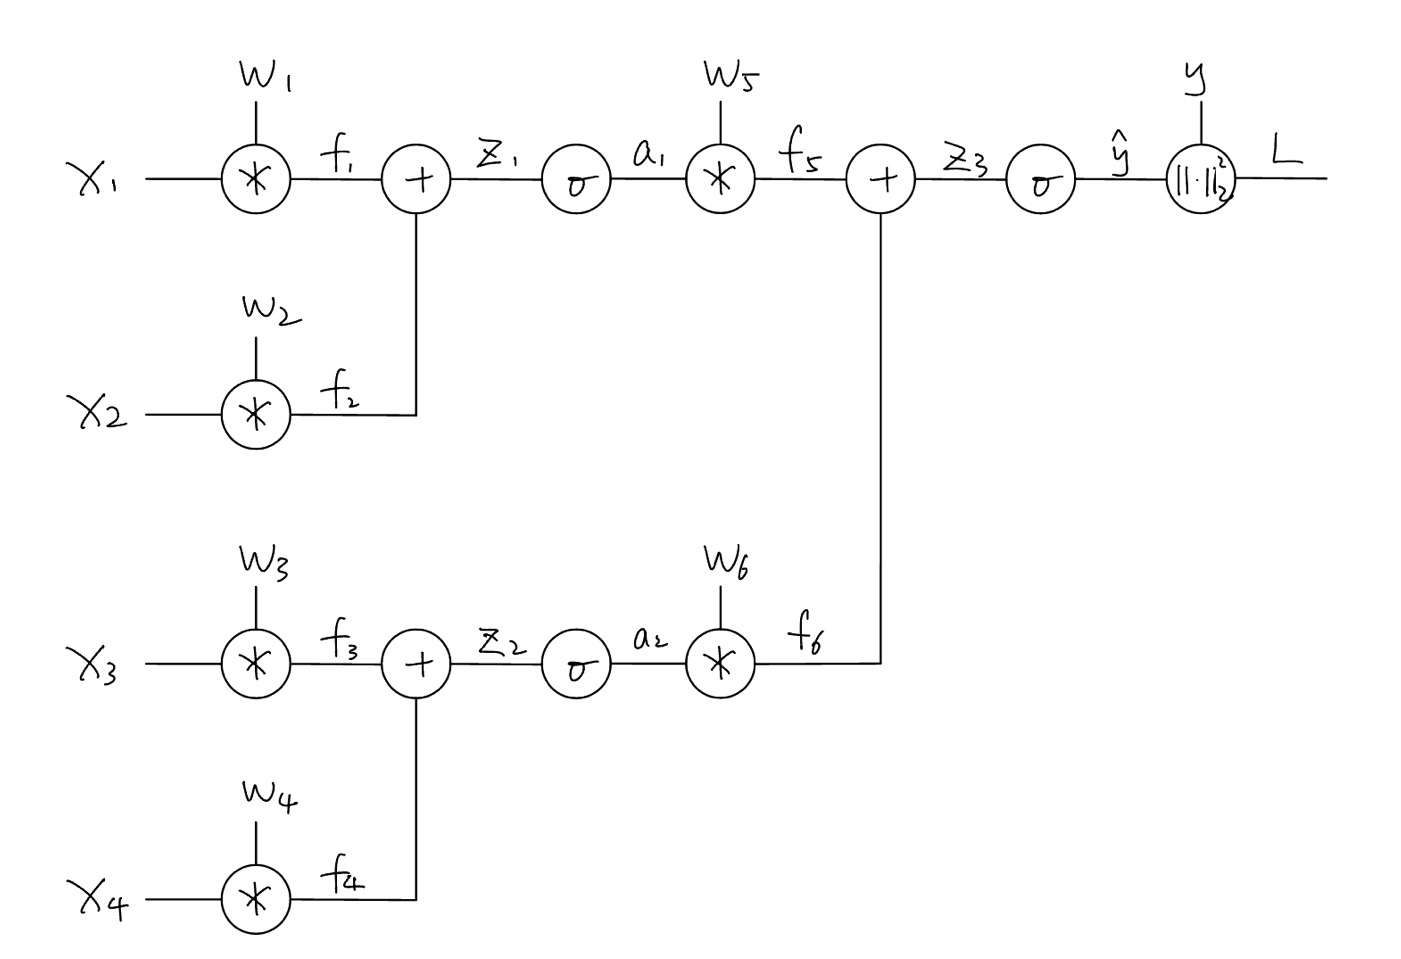
\includegraphics[width=1\textwidth]{q3a.jpg}
\caption{Computational Graph}
\end{figure}

\subsubsection*{3.b:}
Given: 
\(\sigma'(z) = \sigma(z)\,[1 - \sigma(z)]\).  

$\begin{aligned}
\frac{\partial L}{\partial \hat{w_3}}
&= \frac{\partial L}{\partial \hat{y}}
\frac{\partial \hat{y}}{\partial z_3}
\frac{\partial z_3}{\partial f_6}
\frac{\partial f_6}{\partial a_2}
\frac{\partial a_2}{\partial z_2}
\frac{\partial z_2}{\partial f_3}
\frac{\partial f_3}{\partial w_3}\\
&= 2(y-\hat{y}) \cdot \hat{y}(1-\hat{y}) \cdot 1 \cdot w_6 \cdot a_2(1-a_2) \cdot 1 \cdot x_3\\
&= -0.01133375784816148370112714641802\\
&\approx -0.0113
\end{aligned}$\newline\newline
Hence, the final answer (to 4 decimal places) is:
\[
\frac{\partial L}{\partial w_3} \;=\; -0.0113.
\]\newline


\subsection*{Question 4: Convolutional Neural Network}
Layer C input: $50 \times 12 \times 12$\newline
Layer C FLOPS without bias:

$\begin{aligned}
&[\text{(input dimentions)}50 \times \text{(conv cost)}(4 \times 4) + \text{(addition)}(50 \times 4 \times 4 - 1)]\\
&\times \text{(input dimentions)}20 \times \text{(output size)}(6 \times 6)\\
= & [(50 \times 4 \times 4) + (50 \times 4 \times 4 - 1)] \times (20 \times 6 \times 6)\\
= & (1599) \times 720\\
= & 1151280
\end{aligned}$\newline
Layer C FLOPS with bias:

$\begin{aligned}
&[\text{(input dimentions)}50 \times \text{(conv cost)}(4 \times 4) + \text{(addition)}(50 \times 4 \times 4 - 1 + 1)]\\
&\times \text{(input dimentions)}20 \times \text{(output size)}(6 \times 6)\\
= & [(50 \times 4 \times 4) + (50 \times 4 \times 4)] \times (20 \times 6 \times 6)\\
= & (1600) \times 720\\
= & 1152000
\end{aligned}$\newline
Layer P FLOPS:

$\begin{aligned}
&\text{(input dimentions)}20 \times \text{(MaxPool cost)}(9-1) \times \text{(output size)}(4 \times 4)\\
= & 20 \times 8 \times 4 \times 4\\
= & 2560
\end{aligned}$\newline\newline\newline
Total FLOPS without bias: $1151280 + 2560 = 1153840$\newline
Total FLOPS with bias: $1152000 + 2560 = 1154560$\newpage


\subsection*{Question 5: Trainable Parameters}
C1(convolution): $\text{(conv dimensions)}6 \times [\text{(filter size)}(5 \times 5) + 1] = 156$\newline
S2(subsampling): $0$\newline
C3(convolution): $\text{(conv dimensions)}16 \times [\text{(filter size)}(5 \times 5 \times 6) + 1] = 2416$\newline
S4(subsampling): $0$\newline
C5(full): $\text{(input)}(16 \times 5 \times 5 + 1) \times \text{(output)}120 = 48120$\newline
F6(full): $\text{(input)}(120 + 1) \times \text{(output)}84 = 10164$\newline
OUTPUT(full): $\text{(input)}(84 + 1) \times \text{(output)}10 = 850$\newline\newline
Total trainable parameters: $156 + 0 + 2416 + 0 + 48120 + 10164 + 850 = 61706$\newline


\subsection*{Question 6: Logistic Activation Function}
Logistic activation function is defined as:
\[
\sigma(x) = \frac{1}{1+e^{-x}}.
\]
Output of the neuron is
\[
y = \sigma(x).
\]
The derivative w.r.t. the input \(x\) is
\[
\frac{dy}{dx} = \sigma(x)(1-\sigma(x)) = y(1-y).
\]
Thus, for backpropagation, the gradient can be computed using only the output \(y\), without needing the original input \(x\).\newline


\subsection*{Question 7: Hyperbolic Tangent Activation Function}
\subsubsection*{7.a:}
\begin{itemize}
     \item hyperbolic tangent function: \(\tanh(x)\) outputs range: \((-1, 1)\).
     \item logistic activation function: \(\sigma(x)\) outputs range: \((0, 1)\).
\end{itemize}

\subsubsection*{7.b:}
We know:
\[
\tanh(x) \;=\; 2\,\sigma(2x) \;-\; 1.
\]
The derivative expressed using logistic function:
\[
\frac{d}{dx}\bigl(2\,\sigma(2x) - 1\bigr)
\;=\;
2 \cdot \sigma'(2x) \cdot 2
\;=\;
4\,\sigma'(2x).
\]
Since
\[
\sigma'(z) \;=\; \sigma(z)\bigl[1-\sigma(z)\bigr],
\]
we have
\[
\sigma'(2x) 
\;=\;
\sigma(2x)\,\bigl[1-\sigma(2x)\bigr].
\]
Hence,
\[
\frac{d}{dx}\tanh(x)
\;=\;
4\,\sigma(2x)\,\bigl[1-\sigma(2x)\bigr].
\]
Therefore, the gradient of \(\tanh(x)\) can be viewed entirely in terms of \(\sigma(2x)\).

\subsubsection*{7.c:}
\begin{itemize}
     \item Logistic Function:
       \begin{itemize}
         \item Outputs are in \((0,1)\), better for modeling probabilities.
         \item Commonly used in the final layer for binary classification (logistic regression).
       \end{itemize}
     
     \item Hyperbolic Tangent Function:
       \begin{itemize}
         \item Outputs are in \((-1,1)\), centered around 0, better for sigmoid in hidden layers because zero-centered outputs can help
               with faster convergence during backprop.
       \end{itemize}
\end{itemize}\newpage


\section*{Part II: Implementation Tasks}
\subsection*{Task I - Inspection}
Upon inspection, the SDD dataset introduces more variability than the DBI dataset: 
The images in SDD have more diverse dog positions, poses, and background compared to the DBI dataset, which are more centered and have cleaner background.
Also the images in SDD have items(bars, dog toys, people etc.) in view, obscuring parts of the dog.

\subsection*{Task II - simple CNN Training on the DBI}
Plots of traning, test accuracy over 10 epochs, where red line represents the training accuracy, blue line represents the test accuracy.\newline
For training accuracy, the model without dropout could intuitively reach higher training accuracy in the beginning of training, because it is capable to memorize more training examples. However it is affected by the noise of dataset, causing a generally lower accuracy, and fluctuation. \newline
As a generalization to the test set, dropout acts as a regularizer, which helps prevent overfitting, and stabilizes the test accuracy as the training continues.
\begin{figure}[H]
  \begin{minipage}{0.48\textwidth} % Adjust 0.48 for spacing
      \centering
      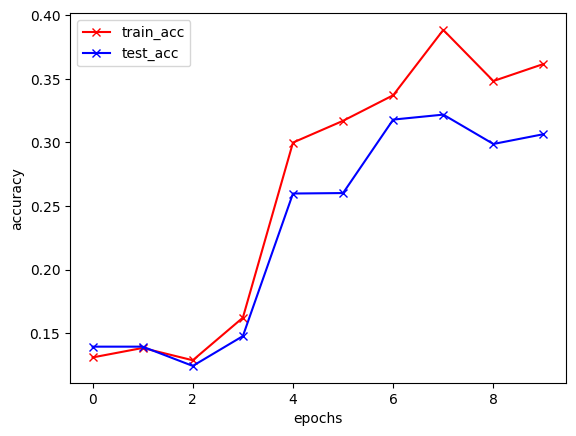
\includegraphics[width=\textwidth]{IIa.png} % Replace image1.png
      \caption{SimpleCNN}
      \label{SimpleCNN}
  \end{minipage}
  \hfill % Fills the space between the minipages
  \begin{minipage}{0.48\textwidth} % Adjust 0.48 for spacing
      \centering
      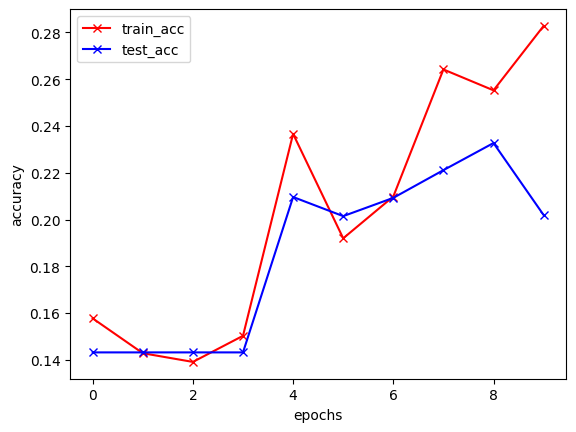
\includegraphics[width=\textwidth]{IIb.png} % Replace image2.png
      \caption{SimpleCNN\_noDropout}
      \label{SimpleCNN_noDropout}
  \end{minipage}
  % \caption{Overall caption for both graphs}
  \label{fig:bothgraphs}
\end{figure}


\subsection*{Task III - ResNet Training on the DBI}
\subsubsection*{III.a:}
Plot of traning, validation, and test accuracy over 10 epochs, where red line represents the training accuracy, green line represents the validation accuracy, and blue line represents the test accuracy.\newline
ResNet18 is a deeper network than the SimpleCNN, it has a higher accuracy than SimpleCNN after 10 epochs of training.\newline
This could be because ResNet18 is typically better at generalizing, thanks to residual connections.
\begin{figure}[H]
  \centering
  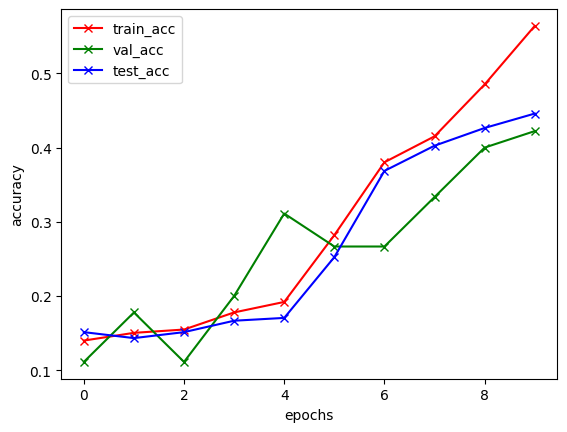
\includegraphics[width=0.6\textwidth]{III.a.png}
  \caption{ResNet18}
\end{figure}

\subsubsection*{III.b:}
\begin{itemize}
  \item DBI Test Accuracy: 0.4459
  \item SDD Test Accuracy: 0.3330
\end{itemize}
The accuracy obtained on the DBI dataset is higher than that of SDD. 
This could be because the model is trained on DBI dataset.
Or that DBI may be a bit easier for the model to classify compared to the SDD test images.
\begin{figure}[H]
  \centering
  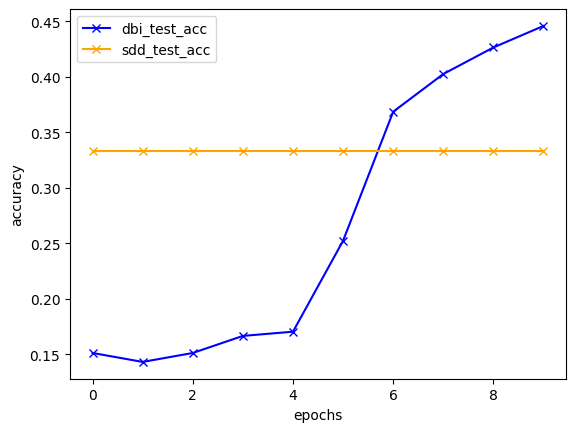
\includegraphics[width=0.6\textwidth]{III.b.png}
  \caption{Comparing Test Accuracy: DBI vs SDD}
\end{figure}\newpage


\subsection*{Task IV - Fine-tuning on the DBI}
Although three models all achieve high accuracy on DBI dataset, 
we can see that ResNeXt32 outperforms ResNet18 and ResNet34 on SDD tesst dataset.\newline
ResNeXt’s higher capacity and higher feature size can adapt better across both datasets, 
while ResNet18 and ResNet34 show a gap in cross dataset 
performance despite high accuracy on DBI.
\begin{figure}[H]
  \begin{minipage}{0.48\textwidth} % Adjust 0.48 for spacing
      \centering
      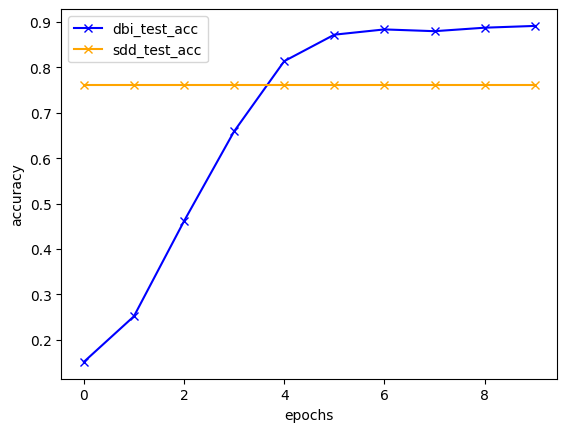
\includegraphics[width=\textwidth]{IV.a.png} % Replace image1.png
      \caption{ResNet18 Test Accuracy: DBI vs SDD}
      \label{ResNet18 Test Accuracy: DBI vs SDD}
  \end{minipage}
  \hfill % Fills the space between the minipages
  \begin{minipage}{0.48\textwidth} % Adjust 0.48 for spacing
      \centering
      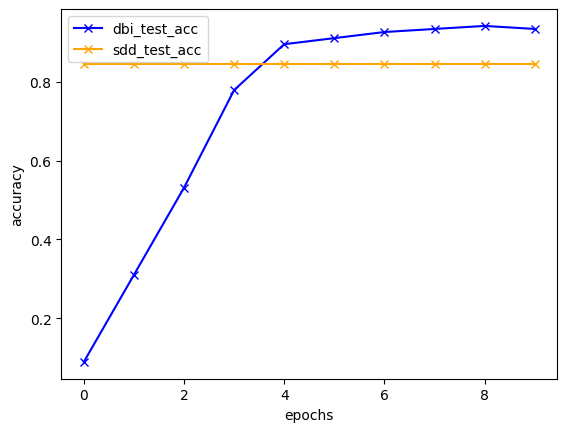
\includegraphics[width=\textwidth]{IV.b.png} % Replace image2.png
      \caption{ResNet34 Test Accuracy: DBI vs SDD}
      \label{ResNet34 Test Accuracy: DBI vs SDD}
  \end{minipage}
  % \caption{Overall caption for both graphs}
  \label{fig:bothgraphs}
\end{figure}
\begin{figure}[H]
  \centering
  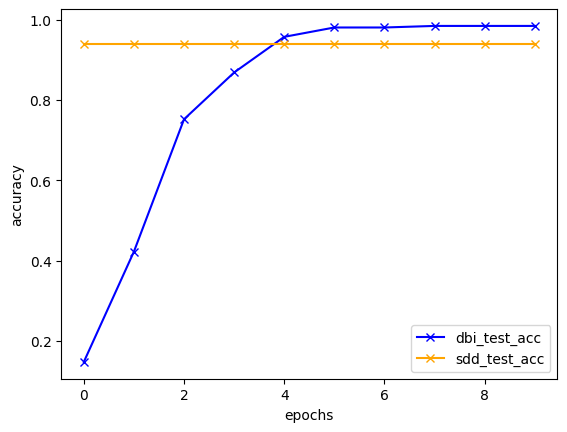
\includegraphics[width=0.48\textwidth]{IV.c.png}
  \caption{ResNeXt32 Test Accuracy: DBI vs SDD}
\end{figure}\newpage


\subsection*{Task V - Dataset classification}
The DatasetClassifier is a fine-tuned model using pre-trained resnext50\_32x4d. 
with last layer adapted to the output size of 2. 
The reason for this pre-trained model is that it gained highest accuracy for classification task in my exploration.
The final test accuracy for this DatasetClassifier: 0.8147.
\begin{figure}[H]
  \centering
  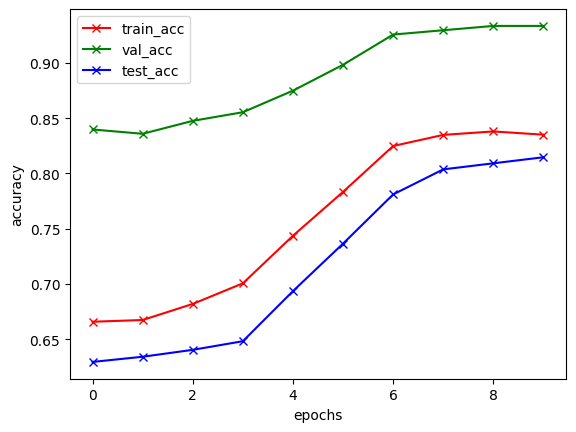
\includegraphics[width=0.6\textwidth]{V.png}
  \caption{DatasetClassifier}
\end{figure}

\subsection*{Task VI - How to improve performance on SDD?}
\begin{itemize}
  \item \textbf{VI.a: Attraining time, we have access to the entire DBI dataset, but none of the SDD dataset. All we know is a high level description of SDD and its differences with DBI (similar to the answer you provided for Task I of this question).}\newline
  More dataset augmentation. Since we know a high level description of SDD and its differences with DBI, we can simulate the known style or conditions of SDD using DBI.
  Use better pre-trained model such as ResNeXt32, which could capture crutial features of the dataset itself, with less bias.
  \item \textbf{VI.b: At training time, we have access to the entire DBI dataset and a small portion \(e.g. 10\%\) of the SDD dataset.}\newline
  Pre-train the model with DBI dataset for general feature understanding, then fine-tune the model using the 10\% SDD dataset for better generalization on SDD dataset.
  \item \textbf{VI.c: At training time, we have access to the entire DBI dataset and a small portion \(e.g. 10\%\) of the SDD dataset but without the SDD labels for this subset.}\newline
  Pre-train the model with DBI dataset. Use predictions of the model on the 10\% SDD dataset as sudo-target for fine-tuning.
\end{itemize}


\subsection*{Task VII - Discussion}
Domain shift (from DBI to SDD) can cause reduced performance or biases in predictions. 
In real-world applications, differences in the settings can lead to biased predictions and low accuracy.\newline
To improve performance to adapt to the domain shift: 
\begin{itemize}
  \item We can add Dropout layers within the model, which could improve generalization and reduce bias in real world setting.
  \item We can Data Augmentation to simulate the setting after the domain shift for better representations of the new setting.
  \item We can Use pre-trained models and apply fine-tuning, so that the model can focus on domain-specific differences, to gained a nuanced conprehension of features.
\end{itemize}




\end{document}
